\documentclass[11pt]{article}

%\usepackage[utf8]{inputenc}\usepackage[T1]{fontenc}
\usepackage{titling}
\usepackage{times}
\setlength{\droptitle}{-5em}   % This is your set screw
\usepackage{ps}
\usepackage{comment}
\usepackage{physics}
\usepackage{setspace}
\usepackage{bbm}
\usepackage{titlesec}
\titleformat{\section}{\large\bfseries}{\thesection}{1em}{}

\DeclareMathOperator{\interi}{int}

\title{\bf\Large{Summary of Multi-Agent Area Coverage Control Using Reinforcement Learning}}
\author{Simon Hu}
\date{}

\begin{document}
\maketitle

\section{Introduction}
% Complete the following section; it is separate from the notational measures. s
Coverage control of mutli-agent systems is concerned with deploying agents over an environment to maximize sensor coverage, for various tasks such as sensing, data collection and surveillance. Consider a group of $N$ homogeneous agents moving in a compact environment $\Omega \subset \R^2$, where the dynamics of the $i$-th agent is given by 
\begin{equation}
	\displaystyle \ddot{p}_i = u_i
\end{equation}
where $p_i = (x_i, y_i) \in \R^2$ represents the agent's location and $u_i = (u_{x_i}, u_{y_i}) \in \R^2$ represents the velocity vector. The goal of solving the coverage control problem is to find a configuration of agent positions, $p = (p_1, p_2, \dots, p_N)$ such that the cost index 
\begin{equation}
	\label{intro:cost index}
	\displaystyle \mathcal{H}(p,t) = \int_{\Omega}{\max\limits_{i=1,2,\dots,N}{f_i(\,\norm{p_i - q})} \phi(q, t) \: \dif q}
\end{equation}
is maximized. In the above, $\phi : \Omega \times \R_{\geq 0} \to \R_{\geq 0}$ is a probability density that represents the probability of an event occuring at point $q \in \R^2$ and $f : \R^2 \to \R$ is a non-increasing Lesbegue measurable function of the distance between points. Intuitively, $\phi$ reflects some measure of the number of agents that need to be deployed to a particular point. The choice of $f$ reflects the sort of coverage task we are attempting to achieve. For maximum area coverage, the function $f(x) = -x^2$ is considered.

A collection $S = (S_1, S_2, \dots, S_M)$ is a partition of $\Omega$ if $\interi(S_i) \cap \interi(S_j) = \emptyset$ (i.e. the sets have disjoint interiors) and $\cup(S_i) = \Omega$ (i.e. the union of the sets is $\Omega$). The Voronoi partition of $\Omega$ is given by $\mathcal{V}s = (\V^1, \V^2, \dots, \V^N)$ where each $\V_i$ is described by 
\begin{equation}
	\displaystyle \V_i = \left\{ q \in \Omega \: | \: \norm{q - p_i} \leq \norm{q - p_j}, \forall j \neq i \right\}.
\end{equation}
Under this partition, the cost index (\ref{intro:cost index}) can be rewritten as 
\begin{equation}
	\displaystyle \mathcal{H}(p,t) = \sum\limits_{i=1}^{n}{\int_{\V_i}{f(\, \norm{q - p_i}) \phi(q, t)\: \dif q}}.
\end{equation}
In this manner, the algorithm is spatially distributed, i.e. each agent only has to use local neighbor information to compute its contribution to the total cost. The mass and center of mass of $\V_i$ are given by 
\begin{align}
	\displaystyle &m_{\V_i} = \int_{\V_i}{\phi(q) \: \dif q}, \:\:\: c_{\V_i} = \frac{1}{m_{\V_i}}\int_{\V_i}{q\phi(q) \: \dif q}
\end{align}
respectively. It is shown in \cite{Nowzari:2012:SCR:2207287.2207546} that the optimal partition of $\Omega$ is the Voronoi partition and the optimal sensor placements, $p$ are the centers of mass of the Voronoi cells. 
\begin{comment}
\begin{equation}
	\displaystyle \dot{e}_i(t) = Ae_i + Bu_i
\end{equation}
where $A$ and $B$ are given by 
\begin{equation}
	\displaystyle A = \frac{2k_p m_{\V_i}}{k_d}\left(\frac{\partial c_{\V_i}}{\partial p_i} - I_2\right), \: \: B = k_d^{-1}\left( I_2 - \frac{\partial c_{\V_i}}{\partial p_i} \right).
\end{equation}
From basic linear systems theory, the system can be written in discrete form, at some discrete step $k+1$, as 
\begin{equation}
	\displaystyle \dot{e}_i(k+1) = A_de_i(k) + B_du_i(k)
\end{equation}
where the matrices $A_d, B_d$ are given by $A_d = \exp(AT)$ and $B_d = \int_{0}^{T}{\exp(A(T - \tau)) Bu(\tau) \: \dif \tau}$ respectively. Here, the discretization is over a time horizion $[0, T]$. Using the LaSalle invariance principle, it can be shown that the feedback law given by (\ref{control law : feedback control}) converges to the centroidal Voronoi configuration. Note that the error dynamical model is not used in the computations. It is only introduced in order to apply the LaSalle invariance principle to show convergence to the centroidal Voronoi configuration. 
\end{comment}
\section{Actor-Critic Neural Network}
Designing a controller that realizes the control law considered in \cite{Cortes:2004} is difficult, so an Actor-Critic Neural Network (ACNN) approximation is employed. Define $e_i(t) = c_{\V_i}(t) - p_i(t)$ as the centroid error for agent $i$ and  consider the Value function at the $k$-th step, given by 
\begin{equation}
	\label{before bellman}
	\displaystyle V(e_i(k)) = \sum\limits_{\kappa = k}^{\infty}{e_i^T(\kappa)Qe_i(\kappa) + u_i^T(\kappa)Ru_i(\kappa)}
\end{equation}
where $Q, R \in \R^{2 \times 2}$ are positive definite matrices. It is important to note that the second term in the Value function quantizes some measure of energy expenditure, which is important for long-term surveillance and data collection tasks. For notational simplicity, let us write $V_{i,k} = V(e_i(k))$. To put the Value function into the form of a Bellman equation, we rewrite (\ref{before bellman}) as 
\begin{equation}
	\displaystyle V_{i,k} = e_i^T(k)Qe_i(k) + u_i^T(k)Ru_i(k) + V_{i, k+1}
\end{equation}
so that the minimization to be solved is 
\begin{equation}
	\displaystyle V_{i,k}^* = \min\limits_{u_i(k)}{\left[e_i^T(k)Qe_i(k) + u_i^T(k)Ru_i(k) + \gamma V^*_{i, k+1}\right]}
\end{equation}
where $\gamma$ is the discount factor. To put this in the language used in the class, we are trying to find the optimal policy $u_i$ that minimizes the value function. To solve this problem, we assume the following structure for the Value function and policy.
\begin{align}
	\displaystyle &\widehat{V}_j(e_i(k)) = w^T_{c, j} \rho(e_i(k)), \:\:\: \widehat{u}_j(e_i(k)) = w^T_{a, j} \sigma(e_i(k)).
\end{align}
Here, $\widehat{V_i}$ and $\widehat{u_i}$ are the estimates of the Value function and policy respectively, $w_{c,j}, w_{a, j}$ are the network weights, and $\rho, \sigma$ are the activation functions of the network. The loss of the critic and actor neural networks are given by 
\begin{align}
	\label{critic loss}
	\displaystyle &E_{c,j} = \frac{1}{2}\sum\limits_{\ell=1}^{N_t}{\left[ w^T_{c,j+1}\rho^\ell(e_i(k)) - V_{i,j+1}^\ell\right]^2}, \:\:E_{a,j} = \frac{1}{2}\sum\limits_{\ell=1}^{N_t}{\left[w_{a,j+1}^T\sigma^\ell(e_i(k)) - u_{j+1}^\ell(e_i(k)) \right]^2}
\end{align}
which is again just the least squares loss. A target and source network is initialized and tracked for both the actor and critic. The weights are synced (i.e. there is a soft update of the weights) to improve numerical stability by using a soft actor-critic update law. 
\begin{comment}
For some hyperparameter $\beta \ll 1$, the soft updates for the actor and critic networks are given by 
\begin{align}
	&w_{a, j+1, t}^T(k) \leftarrow \beta w_{a, j+1, t}^T(k) + (1 - \beta)w_{a, j+1, s}(k) \\
	&w_{c, j+1, t}^T(k) \leftarrow \beta w_{c, j+1, t}^T(k) + (1 - \beta)w_{c, j+1, s}(k)
\end{align}
where the extra subscript is used to differentiate between the target and source network weights (i.e. $t$ for target, and $s$ for source).
\end{comment}
\section{Algorithm}
With very minor modifications, the main meat of the algorithm is the Soft Actor-Critic DDPG algorithm. For more information, consult \cite{deep}.
\section{Simulation Results}
\begin{figure}[H]
	\begin{subfigure}{.5\textwidth}
		\centering 
		\includegraphics[width=.5\textwidth]{config}
		\caption{The final, optimal deployment of five agents in a convex environment with the corresponding Voronoi cells and risk density function $\phi$, in purple.}
	\end{subfigure}
	\begin{subfigure}{.5\textwidth}
		\centering 
		\includegraphics[scale=0.37]{coverage}
		\caption{The percentage of coverage as a function of time. The black line shows the results from \cite{FLAIRS1612802} (i.e. this paper) and the dash red line shows the results from \cite{Cortes:2004}.}
	\end{subfigure}
	\begin{subfigure}{.5\textwidth}
		\centering 
		\includegraphics[scale=0.37]{error}
		\caption{The Euclidean error between each agent and its corresponding centroid.}
	\end{subfigure}
	\begin{subfigure}{.5\textwidth}
		\centering 
		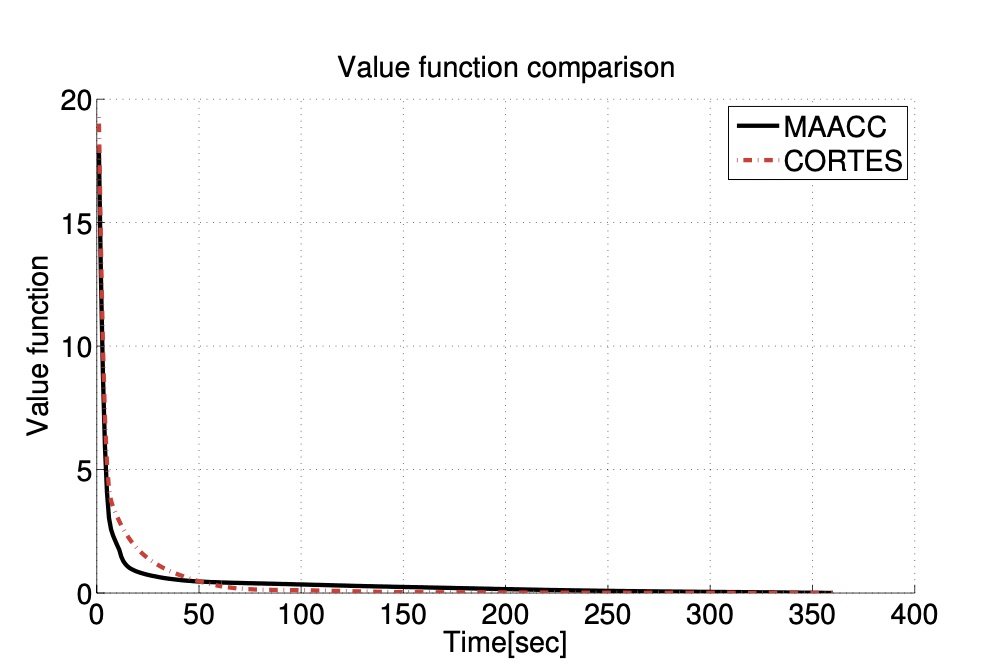
\includegraphics[scale=0.37]{value}
		\caption{The output of the value function. The black line shows the results from \cite{FLAIRS1612802} (i.e. this paper) and the dashed red line shows the results from \cite{Cortes:2004}.}
	\end{subfigure}
\end{figure}
% Generate bibliography.
\bibliography{ref}
\bibliographystyle{ieeetr}
\end{document}